\section{Clouds role in the climate system} \label{sec:cloud_in_climate_system}
% Clouds, climate and machine learning
Clouds play an important role in the climate system both affecting the radiative budget and the hydrological cycle. Understanding how clouds form in the complex system of the atmosphere involves both knowledge about the large scale influence by the circulation and the small scale influence by aerosols. 
%Climate models are the most useful tool for studying the past, present and future climate. Clouds and aerosols are acknowledged as the factors contributing with the largest uncertainty to the \acrfull{ecs}. Also known as global mean temperature increase as a consequence of doubling of the pre-industrial levels of $CO_2$ (280 \acrshort{ppm}). \textbf{kilde AR4 which ch?} \textit{It remains unclear to which level of sophistication is adequate to model their effect om climate.} (\cite{IPCC_CH7_clouds}).
%\newpage
\subsection{Evolution of clouds}
Clouds are composed of liquid droplets, ice crystal or both. To this day the microphysics of all phases are not fully understood \textcolor{red}{kilde? Her kommer du med en påstand}. Here mixed phase clouds, consisting of both liquid and ice, shows to be the most difficult to fully understand. 

\textit{Aerosols} include both gases and solid particles suspended in the air. They interact with the clouds by serving as particles which vapour and ice can condensate or deposit upon. The different phases require different properties and the nuclei are called \acrfull{ccn} for liquid droplets and \acrfull{inp} for ice crystals. 
\textcolor{red}{Kanskje du burde definere aerosoler først siden du bruker order aerosoler for å forklare hvordan skyer dannes også definere saturation? og det passer bedre med avsnittet under også?}



In this context, \textit{saturation} describes the equilibrium state between to phases \textcolor{red}{er dette en definisjon du selv har funnet på? Eller har det fra et sted? }. For water and vapour it has equal rates of condensation and evaporation. Phase changes occurs when the system deviates from the equilibrium state. Under supersaturated conditions, the rate of condensation exceeds the rate of evaporation, facilitating vapour to condense onto suitable aerosols and initiating the formation of clouds. 
% The energy barrier needed to overcome (surface tension) to homogeneous nucleation 

Saturation is usually achieved by a temperature decrease in rising air masses. The saturation vapour pressure, $e_s$\textcolor{red}{,} is the quantity describing the amount of vapour air can retain at a certain temperature. The ratio at which $e_s$ depend on the temperature, $T$, is described by the Clausius-Clapeyron equation for water, see Equation \eqref{eq:clausius_clapeyron_differentias}. The entalphy of vaporization, $l_v$\textcolor{red}{,} is the amount of energy needed to evaporate one unit (e.g one mole) of molecules from the liquid. This is also known as the latent heat of vaporization. 
\begin{equation} \label{eq:clausius_clapeyron_differentias}
    \frac{de_s}{dT} = \frac{l_v e_s}{R T^2}
\end{equation}
Here $l_v = 40.8 \cdot 10^3 J mol^{-1}$ and the universal gas constant $R= 8.314 J mol^{-1} K^{-1}$ (\cite{cloud_phys_book_johanne}, p. 42). 

The solution to Equation \eqref{eq:clausius_clapeyron_differentias}, shown in Equation \eqref{eq:clausius_clapeyron}, is derived by integrating from $T_0 = 273.15K \left(0 ^{\circ}C \right)$ to a arbitrary temperature, $T$. The integral is intractable for varying $l_v$, however a constant $l_v$ is in most cases a reasonable assumption for the ranges of temperatures in atmospheric interest.

The lower boundary, $T_0$, is chosen based on convenience, motivated by the fact that the constant of integration,  $e_0$, needs to origin from measurements. At $T_0$, the equilibrium of a mixture of water and ice at a total pressure of $1$ $atm$ is $e_0 = 611Pa$. 

\begin{equation} \label{eq:clausius_clapeyron}
    e_s\left( T \right) = e_0 e^{\frac{l_v}{R} \left( \frac{1}{T_0} - \frac{1}{T} \right) }
\end{equation}
From Equation \eqref{eq:clausius_clapeyron} it is clear that the $e_s$ increase with rising temperature, resulting in the phenomena that warmer air retain more vapour. The same principles apply for the phase change sublimation, but its entalphy, $l_s$, has a distinct value (\cite{cloud_phys_book_johanne}, p.135). The saturation vapour pressure with respect to ice, $e_i$, can be derived by replacing $l_v$ by $l_s$.

The reverse process results in cloud dissipation. Subsaturated conditions cause the cloud liquid water to evaporate, and the cloud disappears. 

%From Equation \eqref{eq:clausius_clapeyron} it becomes clear that the  is inversely proportional with the second power of the temperature, meaning that for decreasing temperatures the vapour pressure 
%Double check if this id only valid for adiabatic processes, is there any other assumptions..?
%$R^*$ is the specific gas constant (the universal
%gas constant divided by the mean atmospheric molecular
%weight).  
Growth processes are phase dependant. Liquid droplet grows by diffusion and later by collision and coalescence. At temperatures around -38 $^oC$ (\cite{lohmann2016}) droplets spontaneously freeze and can act as \acrshort{inp}. Clouds consisting purely of ice crystals first grow by deposition of vapour then by aggregation (\cite{Fowler1996LiquidAssumptions}). In the presence of both phases, Wegeron-Bergeron-Findeisen process describe the mechanism where droplets evaporate and deposit on to the ice crystals. %When both phases are present in a cloud, the saturation vapour pressure over ice is higher than over liquid. This may cause the droplets to evaporate and deposit on to the ice crystals. 
This mechanism exist because the saturation vapour pressure is lower with respect to ice than water, $e_i < e_s$. It is most efficient at -12$^{\circ}C$ when the difference is largest.

%\section{Clouds role in the energy budget}

\subsection{Clouds role in the radiative budget}
The characteristic white colour of the clouds has it nature in its ability to  effectively scatter solar radiation. %(explains why they appear white - because the backscatter radiation of all wavelenght in the visible spectrum)
%In part, this mechanism describes the important role in the Earth radiative budget. 
The Earth bathes in radiation from the Sun. Passing through the atmosphere, a small portion of the stream gets absorbed. Another portion falls victim to scattering by clouds \textcolor{red}{punktum? Skjønte ikke helt setningen}%gets is scattered by clouds. 
The majority of the radiation reach the Earth and transforms into heat, warming the surface \textcolor{red}{"The majority of the radiation reaches the Earth and transforms into heat, warming the surface"}. The Earth emits thermal radiation, a minor portion of this escape directly back to space, most of it gets absorbed by the atmosphere and is reemitted. This phenomena is know as \textit{the greenhouse effect}. The amount of heat trapped in the Earth system depends fundamentally on the spectral properties of its components (i.e. clouds, greenhouse gases, aerosols), and determines the magnitude of the enhanced warming (\cite{greenhouse_effect}).
\textcolor{red}{Snakket med Katie og det er ikke vanlig å bruke "Earth" eller "Sun" med mindre det er navnet på planten ellers hvsi det er objekter/intetkjønn burde man bruke liten bokstav. Så her får du føle deg frem :)}

\textbf{This was originally placed in the next section after describing the cloud radiative effect, but I thought it might be more suitable here since general. How clouds play a role in the climate system. comments please}

The physical properties causing the interaction with radiation is described below \textcolor{red}{Rar overgang. Kanskje du bare kan lage en litt mer generell beksirvelse som gir en bedre overgang? SKal tenke litt mer på denne}. Dense low level clouds reflect solar radiation \textcolor{red}{Du skrev over at noe ble "scattering by clouds". Betyr denne setningen at det bare er lave skyer som reflekterer eller at det er skyer generelt, men mest de lave? }. This is called the albedo effect. \textit{Albedo} being the ratio between reflected to incoming radiation. Higher number concentrations of droplets, leads to a increase in accumulated surface area, consequently more radiation is reflected back into space. \textcolor{red}{Foretrekker at definisjonen kommer først, men det er kanskje bare meg. }

\textcolor{red}{Hva med: \textit{Albedo} is the ratio between reflected to incoming radiation. Higher number concentrations of droplets, leads to a increase in accumulated surface area, consequently more radiation is reflected back into space. Dense low level clouds reflect solar radiation..... Og her må du knytte det til albedo på et vis}

The greenhouse effect of clouds follows the principals of the general greenhouse effect. It arise from their ability to absorb thermal radiation and reemit it. The absorbed radiation originates from the surface, a widely used assumption is that the Earth radiates like a black body, thus its radiant flux is given by Stefan-Boltzmann forth-power law, 
\begin{equation} \label{eq:stefan-boltzmann}
    F = \sigma  T ^4 % \epsilon
\end{equation}
here $F$ denotes flux in units of $W m^{-2}$, $T$ denotes temperature in units of $K$ and \\  $\sigma = 5.670 \time 10^{-8} W m^{-2} K^{-4}$ is the Stefan-Boltzmann constant. 

The \textit{emissivity}, $\epsilon$\textcolor{red}{,} of a medium is the ratio between the actual emission and the black body emission at the same temperature. It depends on the beams frequency and the viewing angle. Most models assume a black body emission of \textcolor{red}{the} Earth and the atmospheric components, this corresponds to a emissivity, $\epsilon=1$. This provides an additional source of uncertainty to the computations of the greenhouse effect of clouds and therefore also the \acrshort{ecs}.

Mediums like water, snow and ice are not perfect emitters, this requires the need for modifying Equation \eqref{eq:stefan-boltzmann} with a scaling factor, called emissivity, $\epsilon \in [0, 1]$, this depends on the composition, compactness and surface roughness of the medium. The emitted flux is given by $ F = \sigma \epsilon T ^4$. 

    To asses the validity of the black body assumption on the Earth surface\textcolor{red}{,} \citeauthor{Huang2018ImprovedClimate} \textcolor{red}{(\citeyear{Huang2018ImprovedClimate})} demonstrated the changes in the radiative transfer calculations by varying the emissivity based on surface types. Their findings show that it makes a considerable change to the radiative transfer calculations, and in conclusion it need to be further investigated. Researchers are still struggling with determining the exact spectral emissivity of different mediums. This is of interest for both implications to the radiative transfer calculation, but it is also of utmost importance in the field of remote sensing, where distinguishing the signal from the reference signal continue to pose as a problem.
%this property is also being exploited in remote sensing. In remote sensing it is of utmost importance to distinguish the signal from the reference signal, a cloud from its background for instance. 
%Different parts of the globe are covered by different surfaces and \citeauthor{Huang2016AnSimulations} proved that assuming a constant surface emissivity effects the \acrfull{toa} polar energy budget \textbf{read paper again to determine why this is of importance}. 

The greenhouse effect increases with the cloud altitude, enhanced by the temperature difference between the surface and cloud increase \textcolor{red}{Blir det mer riktig å si "...the surface and increase of cloud altitude"?}. High clouds with low temperatures and reemitted radiation at a lower intensity than they absorbed, this has a warming effect \textcolor{red}{HEr er det vanskelig å si om du mener at det er høyde skyer OG stråling som reemitteres ... som gir en varmende effekt ELLER om det er høye skyer som rememitterer stårling .... som har en varmende effekt. }. 
%Despite the uncertainties related to emissivity of the medium, the re-emitted radiation is of a lower intensity than what it absorb.
%This is shown in equations \eqref{eq:cre_sw} and \eqref{eq:cre_lw}. \textbf{drop equations..?}

\textit{Global radiative equilibrium} is reached when the temperature of the atmosphere is adjusted such that the radiation emitted to space is equal to the portion absorbed by the surface.



\section{Clouds in the current climate} \label{sec:intro_cloud_current_climate}
\textcolor{red}{Ville lagt inn tekst før bildet. }
\begin{figure}[ht]
    \centering
    \definecolor{mygray}{gray}{0.8}

    \begin{tikzpicture} %[remember picture,overlay]
        \node at (current page.center) {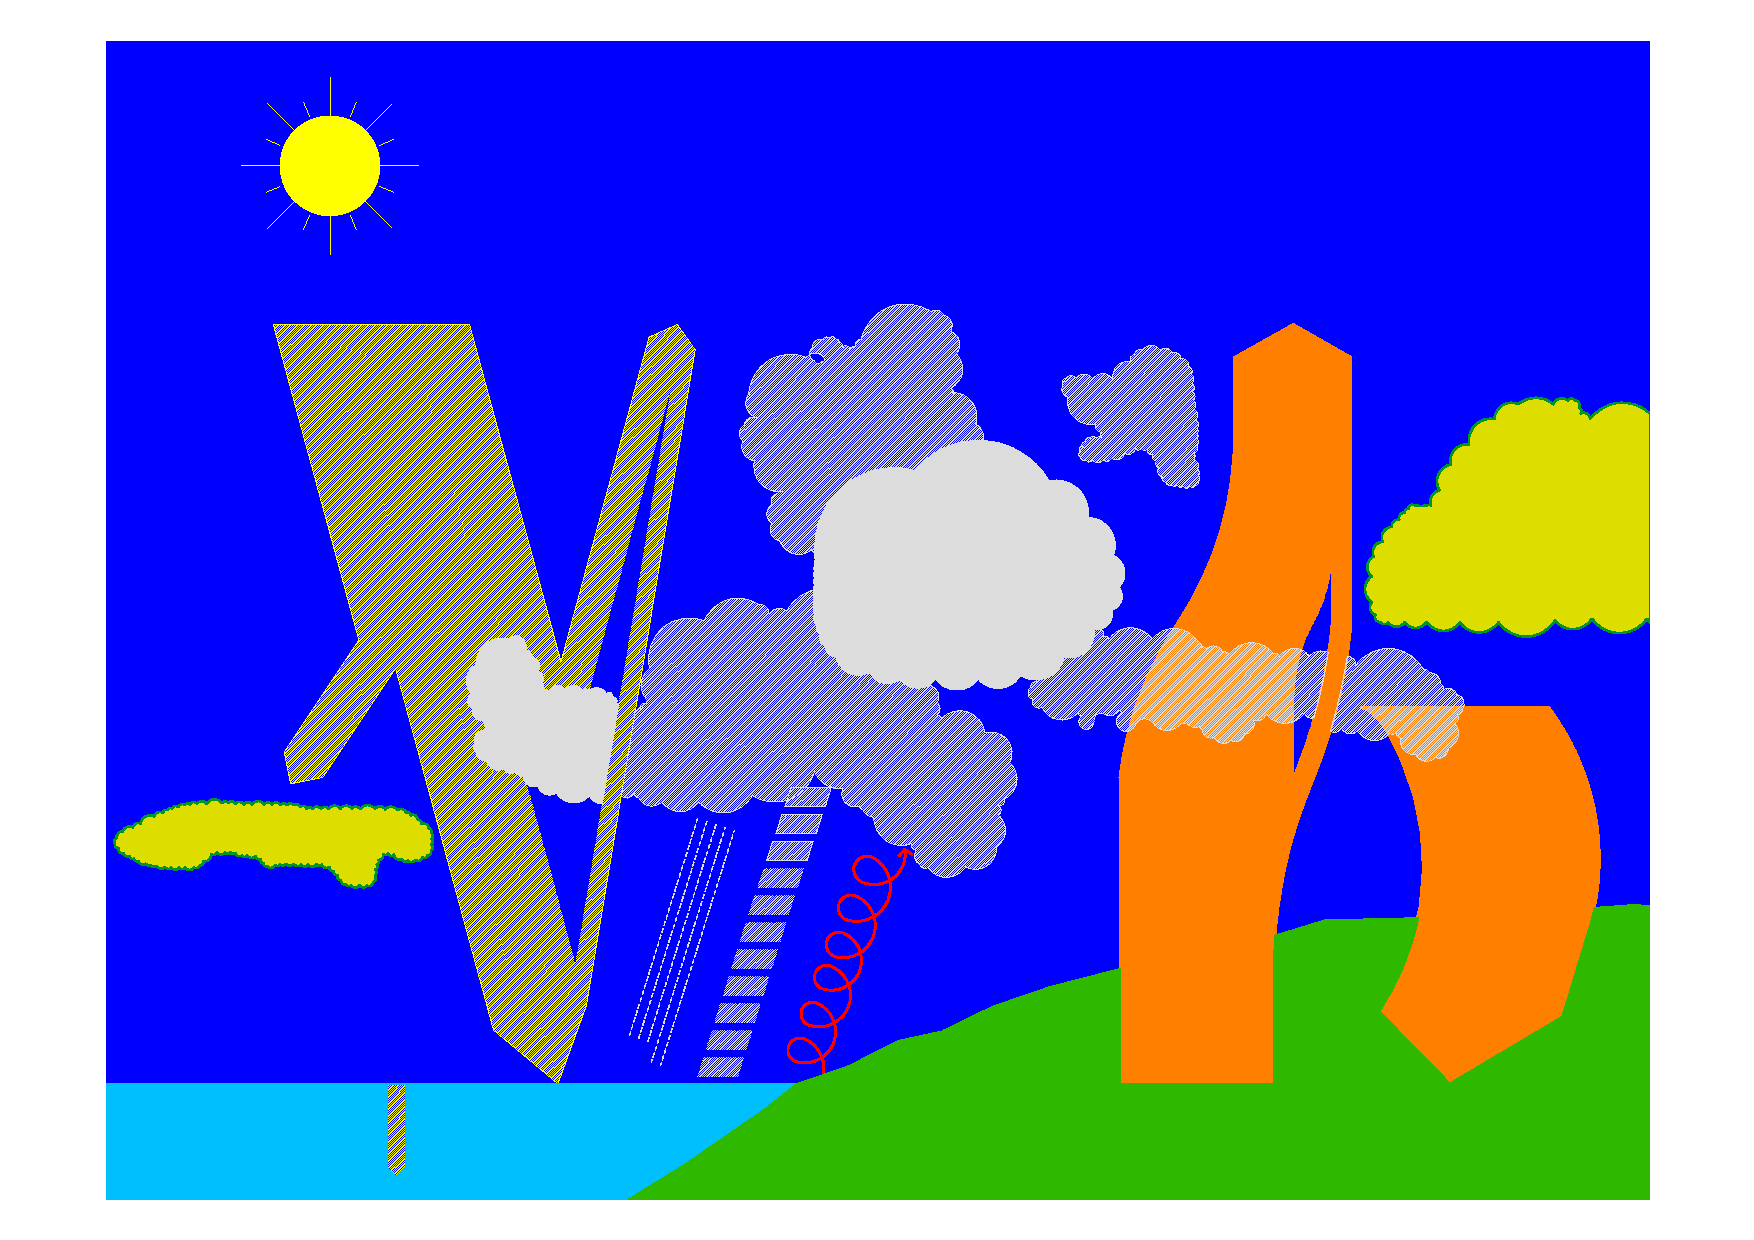
\includegraphics[scale = 0.55]{Chapter2_Theory/images/cre_ny_farge.pdf}};
        \begin{scope}
            % Grid to help find the positions (remove in final version)
            \node at (11cm, 19.5cm) {\Large \textcolor{mygray}{Cloud Radiative Effect (CRE)}};
            
            \node at (14.2cm, 18.1cm) {\Large \textcolor{orange}{LW CRE = +28}};
            %\node at (14.7cm, 16cm) {\large 28};
            
            \node at (9cm, 18.1cm) {\Large \textcolor{yellow}{SW CRE = -47}};
            %\node at (8.7cm, 16cm) {\large -47};
            
            
            % Litt usikker på om jeg syns de bidro
            %\node at (16.5cm, 15.4cm) {\large Atmosphere};
            %\node at (17cm, 18cm) {\large TOA};
            %\node at (16.4cm, 10.2cm) {\large Surface};
            
            \node [rotate = 70] at (10.5cm, 11.6cm) {\small \textcolor{red}{sensible heat}};
            \node [rotate = 73] at (9.7cm, 11.7cm) {\small \textcolor{mygray}{latent heat}};
            \node [rotate = 73] at (8.9cm, 11.5cm) {\small \textcolor{mygray}{solar reflected surface}};
            
            \node at (6.1cm, 10.7cm) {\small Imbalance};
            
            \node at (15.9cm, 11.2cm) {\Large 28};
            \node at (15.4cm, 14.1cm) {\Large 0};
            \node at (7.cm, 14.2cm) {\Large 7};
            \node at (11.2cm, 13.2cm) {\Large 7};
            
            \node at (11.3cm, 15.4cm) {\Large NET CRE};
            \node at (11.3cm, 14.9cm) {\Large =-19};
            
            \node at (11.cm, 10.6cm) {\Large -26};
             
            \node at (16.cm, 10.4cm) {\small thermal};
            \node at (16.cm, 10.1cm) {\small down};
            \node at (16.cm, 9.8cm) {\small surface};
            
            \node at (13.5cm, 11.4cm) {\small thermal};
            \node at (13.5cm, 11.1cm) {\small up};
            \node at (13.5cm, 10.9cm) {\small surface};
            
            \node at (7.6cm, 10.4cm) {\small solar}; % down surface
            \node at (7.6cm, 10.1cm) {\small down};
            \node at (7.6cm, 9.8cm) {\small surface};
            \node at (7.3cm, 11.3cm) {\textcolor{black}{\large -54}};
            
            \node at (5.9cm, 17.4cm) {\small incomming};
            \node at (5.9cm, 17.2cm) {\small solar};
            \node at (5.9cm, 16.90cm) {\small TOA};
            
            \node [rotate = 75] at (8.1cm, 16.cm) {\small solar reflected TOA};
            
            \node at (14.4cm, 17cm)   {\small thermal};
            \node at (14.4cm, 16.7cm) {\small outgoing};
            \node at (14.4cm, 16.4cm) {\small TOA};
            
            \node at (4.7cm, 13cm) {\small \textcolor{black}{solar absorbed}}; % atmosphere
            %\node at (4.38cm, 13.5cm) {\small \textcolor{black}{absored}}; % atmosphere
            \node at (4.6cm, 12.7cm) {\small \textcolor{black}{atmosphere}}; % atmosphere
        \end{scope}

    \end{tikzpicture}
    \caption{The global mean annual \acrfull{cre} is the difference between the radiative components of the clear-sky (cloud-free) and all-sky (cloudy) radiative components. A positive sign can be describes a warming effect and negative a cooling, units in $W m^{-2}$. Inspired by Figure 15 in \citepaper{Wild2019TheModels}.}
    \label{fig:cre}
\end{figure}
%%%%%%%%%%%%%%%%%%%%%%%%%%%%% WILD FIGURE 
%\begin{figure}[h]
%    \centering
%    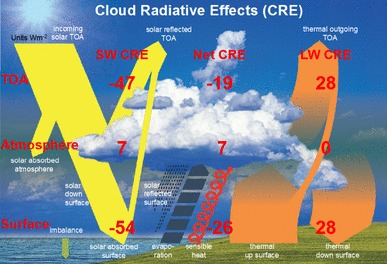
\includegraphics[scale = 7]{Chapter1_Intro/images/CRE_wild2019.jpg}
%    \caption{The global mean annual \acrfull{cre} is the difference between the radiative components of the clear-sky and all-sky radiative components. A positive sign can be describes a warming effect and negative a cooling, units in $W m^{-2}$. This schematic is a modified version of Figure 15 in \cite{Wild2019TheModels}.
%    }
%    \label{fig:cre}
%\end{figure}
On the basis of simulations and available observational data, both remote sensed and in-situ measurements, \citeauthor{Wild2019TheModels}  \textcolor{red}{(\citeyear{Wild2019TheModels})} have quantified the contribution of elements in the Earth\textcolor{red}{s?} annual global mean energy budget. Cloud radiative effect (\acrshort{cre}) is computed by subtracting the components of a cloudy \textcolor{red}{atmosphere} from a cloud-free atmosphere (Ramanathan, 1989?). The altitude along with the composition \textcolor{red}{of the atmosphere?} determines the optical properties of the cloud and in terms its interactions with radiation.

Figure \ref{fig:cre} shows a schematic of the \acrshort{cre} in \textcolor{red}{the} Earths annual mean energy budget, a negative sign denotes a cooling effect and a positive sign can be associated with a warming effect, units are in $W m^{-2}$ \textcolor{red}{Ville droppet "schematic" eller skrevet om til "...shows a schematic illustration of the \acrshort{cre} in...". ville også droppet den siste leddsetningen med "units are in $W m^{-2}$
" da setningen blir veldig lang. Du kan droppe det da det også står i figurteksten, ellers så kan du prøve å legge det inn "...Earths annual mean energy budget (units $W m^{-2}$)...."}. \citeauthor{Wild2019TheModels} \textcolor{red}{(\citeyear{Wild2019TheModels})} finds a reduction in solar radiation of $-47Wm^{-2}$ caused by clouds. Showing that clouds reflect approximately 50\% of the incoming solar radiation. The thermal radiation emitted by clouds amount to $28Wm^{-2}$. Resulting in a net \acrshort{cre} of $-19Wm^{-2}$. Proving that the net effects of clouds on the radiative budget is negative, and that clouds currently have a cooling effect on \textcolor{red}{the} climate. For the details on the all-sky (cloudy) and clear-sky (cloud-free) energy budgets, used to compute the \acrshort{cre}, please see the paper (\cite{Wild2019TheModels}) \textcolor{red}{"please see the paper \citeauthor{Wild2019TheModels} (\citeyear{Wild2019TheModels})}. %\textit{The cloud-free global energy balance and inferred cloud radiative effects: an assessment based on direct observations and climate models} by \cite{Wild2019TheModels}.

%Dense low level clouds reduce the amount of solar radiation absorbed by the surface, and the altitude of the clouds determine the amount of heat trapped in the system. 

\section{Clouds in future climates} \label{sec:intro_cloud_future_climates}
\begin{figure}[h]
    \centering
    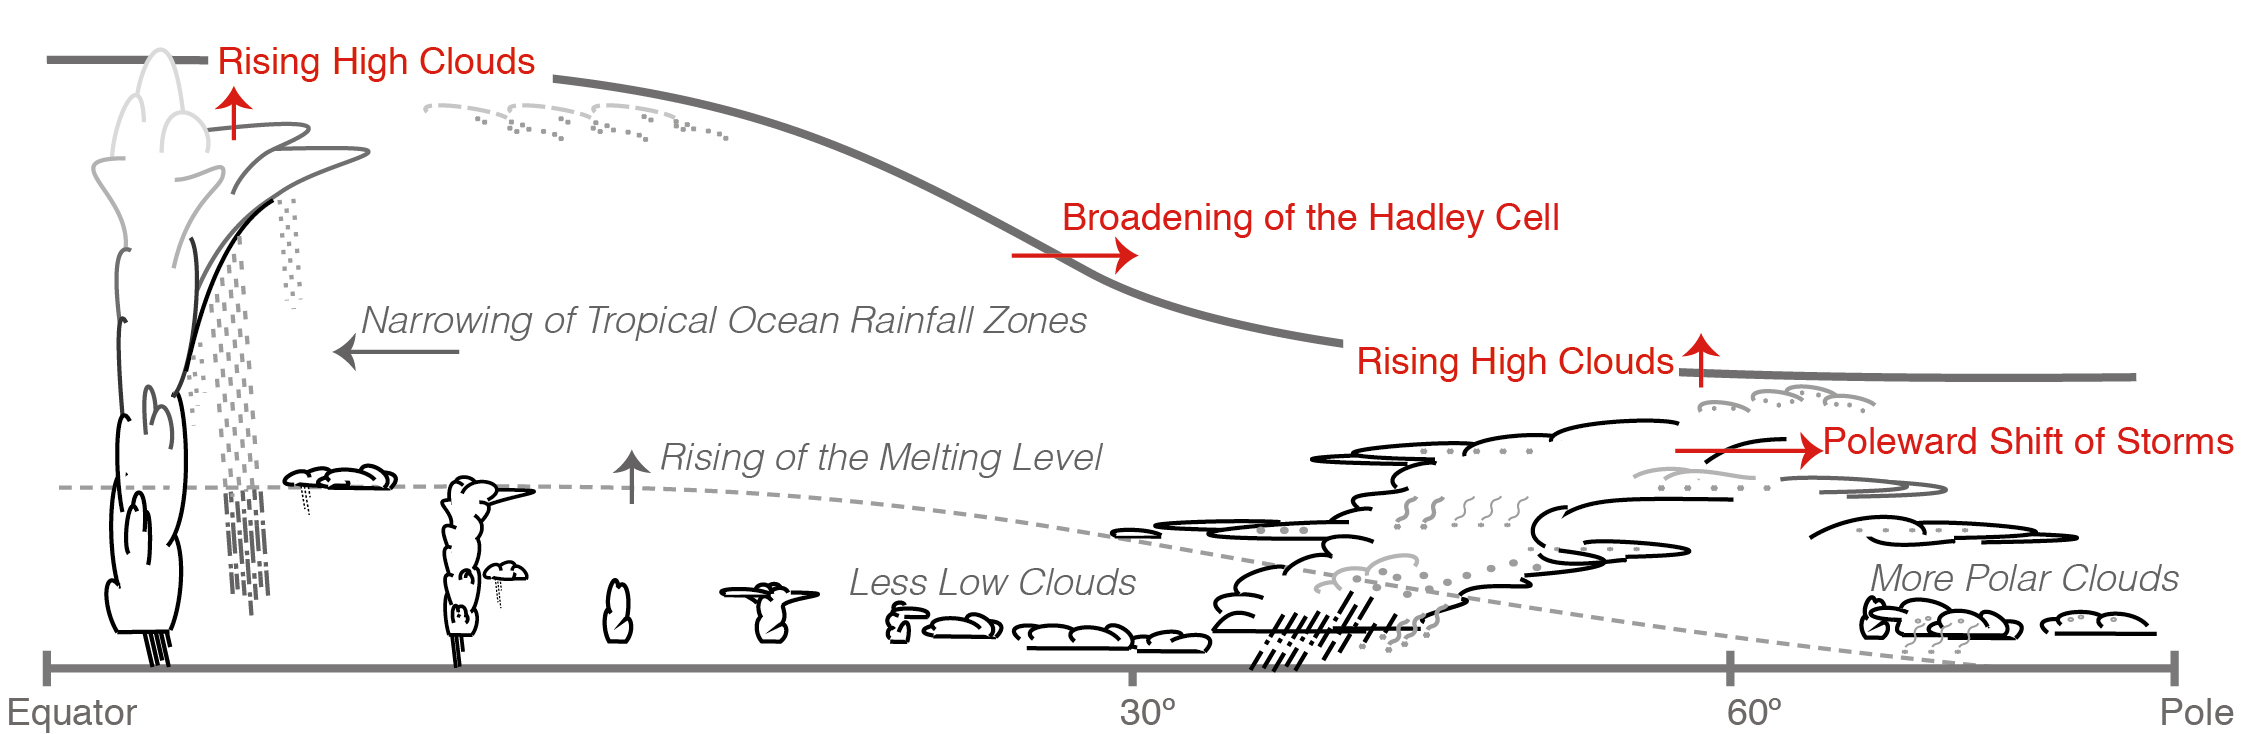
\includegraphics[scale = 0.8]{Chapter1_Intro/images/Fig7-11_ipcc.jpg}
    \caption{Cloud climatology in future climate. Developed based feedback's in climate models, the different adjustments is associated with levels of confidence.  (\cite{IPCC_CH7_clouds}).}
    \label{fig:cloud_scheme}
\end{figure}
As concluded in the previous section, an excess of radiation gets trapped in the Earth system, forcing the atmospheric temperature to increase in order to close the radiative budget. The temperature increase induces climate change and resent estimates finds the imbalance at \acrshort{toa} to be $0.6 Wm^{-2}$ (\cite{Wild2019TheModels}).

% Wild et. al. 2019  \textbf{siter} finds an imbalance of This heat gets trapped in the earth system, forcing the surface temperature to increase in order to close the radiative budget. 
%The imbalance in the radiative budget at \acrfull{toa} is the radiative forcing. 
Climate drivers include both natural and anthropogenic forcings. A \textit{forcing} can be everything from natural variability in the solar energy output, volcanic eruptions or greenhouse gas emissions. The climate science community works toward a common goal to determine the \acrshort{ecs} as a function of forcing. %Different emission scenarios result different \acrshort{ecs}.  

Figure \ref{fig:cloud_scheme} shows a summary of the most likely cloud feedback's, this is the shift in cloud regimes suggested by the \acrshort{ipcc} (\cite{IPCC_CH7_clouds}). \textcolor{red}{To forskjellige setninger. "Figure \ref{fig:cloud_scheme} shows a summary of the most likely cloud feedback's and the shift in cloud regimes suggested by the \acrshort{ipcc} (\cite{IPCC_CH7_clouds})."}

First, a broadening of the Hadley cell causes a poleward shift of storms. This dries up the subtropics and moistens the higher latitudes. Northward propagating clouds would explain a reduction in the albedo effect, caused by the spherical geometry of the Earth, the solar radiation available for reflection decrease poleward, until it disappears into the polar night \textcolor{red}{Altfor lang setning. Kanskje: "Northward propagating clouds would explain a reduction in the albedo effect
. This is because/(as a concequence of)  the spherical geometry of the Earth decrease the solar radiation available for reflection poleward. Leading to a heating in the Arctics/at the poles as a consequence of/as as result of the greenhouse effect of clouds still persist without sunlight." Vet ikke om dette ble noe bedre, men jeg kan prøve å tenke litt videre på den. Den burde det uansett gjøres noe med :)}. 
%proportional with the $sin\left(\theta \right)$, where $\theta$ describes the latitude. 
The greenhouse effect of clouds still persist without sunlight leading to a heating in the Arctic \textcolor{red}{Er det ikke "Arctics"? Altså polene, eller er det bare nordpolen?}.

Second, ascending higher clouds motivate a stronger greenhouse effect. Third, a reduction in the presence of low level clouds reduce the amount of reflect\textcolor{red}{ed?} solar radiation. This is assumed to be partly offset by a\textcolor{red}{n} increase in the melting layer. Rising of the meltlayer cause ice crystals to melt, this phase transition results in more opaque clouds. These have a higher albedo and reflect more sunlight. \textcolor{red}{Forslag: " The reduction of solar radiaton is assumed to be partly offset by an increase in the melting layer. Consequently, the ice crystals melt and the phase transition results in more opaque clouds. ELLER   Causing/Generate/Induce the ice crystals to melt and the phase transition results in more opaque clouds. ELLER Give rise to the melting of the ice crystals inducing phase transition and again more opaque clouds".}